\section{Introduction}
In this report we look to analysis a geothermal heat pump system. First we must understand all the components and how each part interacts with the rest of its system. This paper will first give a brief overview of the different components, the different type of underground loop systems on the market, and then finally address the heat transfer problem with the underground loop systems.
%
\section{Standard Heat Pump System}
A normal heat pump cooling system fitted on most houses uses the vapor compression cycle for cooling and heating. This cycle allows for the removal of heat from one source and the exchange of that heat into a secondary environment. During the summer a house cooling system is removing heat from the inside and dumping it outside. The opposite is true for a house heating system during the winter. When looking at the components of the vapor compression cycle there are four basic parts: a condenser, evaporator, compressor, and expansion valve.
%
\begin{figure}[!tbph]
  \centering
  \subfloat[Example vapor compression cycle with components. \textit{Wikimedia Commons \cite{WikiRefrigeration}}]{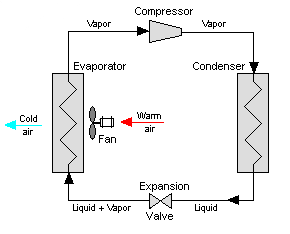
\includegraphics[width=0.4\textwidth]{pictures/Refrigeration.png}\label{fig:f1}}
  \hfill
  \subfloat[Pressure verses specific volume of working fluid inside compression loop. \textit{Wikimedia Commons \cite{WikiRefrigerationPV}}]{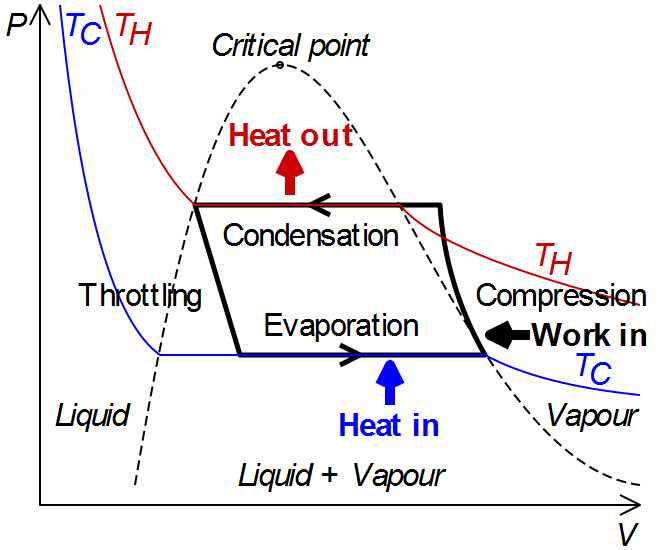
\includegraphics[width=0.4\textwidth]{pictures/Refrigeration_PV_diagram.png}\label{fig:f2}}
\end{figure}
\setcounter{figure}{2}
%
\\
\noindent
By following the refrigerant liquid around the loop we can look at the impact of each component. First the pressure is increased by the compressor doing work on the fluid. This increases the internal temperature of the working fluid and converts it into pressured gas. Then the fluid is put through a condenser which removes this heat and condenses the gas back down to a saturated liquid. After going through an expansion valve to drop the pressure and thus lowering the overall temperature, the fluid can go through another heat exchanger called a evaporator which adds heat from and environment. This cycle can be repeated as long as work, in most cases electricity, is applied to the compressor. During summertime operations, the evaporator is run indoors and the heat from the indoors is ``dumped'' into hotter outside. During the winter heat is extracted from the outside and then ``dumped'' into the indoors through the condenser.
%
%
\section{Geothermal Heat Pump System}
Geothermal heating systems look to replace one of the components in the standard vapor compression cycle. In this case geothermal replaces the standard condenser with its own. Most heat pump systems have their condenser sitting on the outside of the house where the coolant is run through finned coils with fans that blows air over it to exchange the heat with the outside air. Geothermal on the other hand looks to replace this with a underground system of loops. Intuitively one would think that the earth will not be affected as much to the weather, seasons, and air temperature on the surface. It is shown that the ground below the frost layer is on average a constant 13-22 degrees Celsius year around \cite{NRCSScan}. The thought process is that there is a energy ``sink'' in the ground that provides a constant temperature no matter what the outside temperature is.
%
\begin{figure}[H]
    \centering
    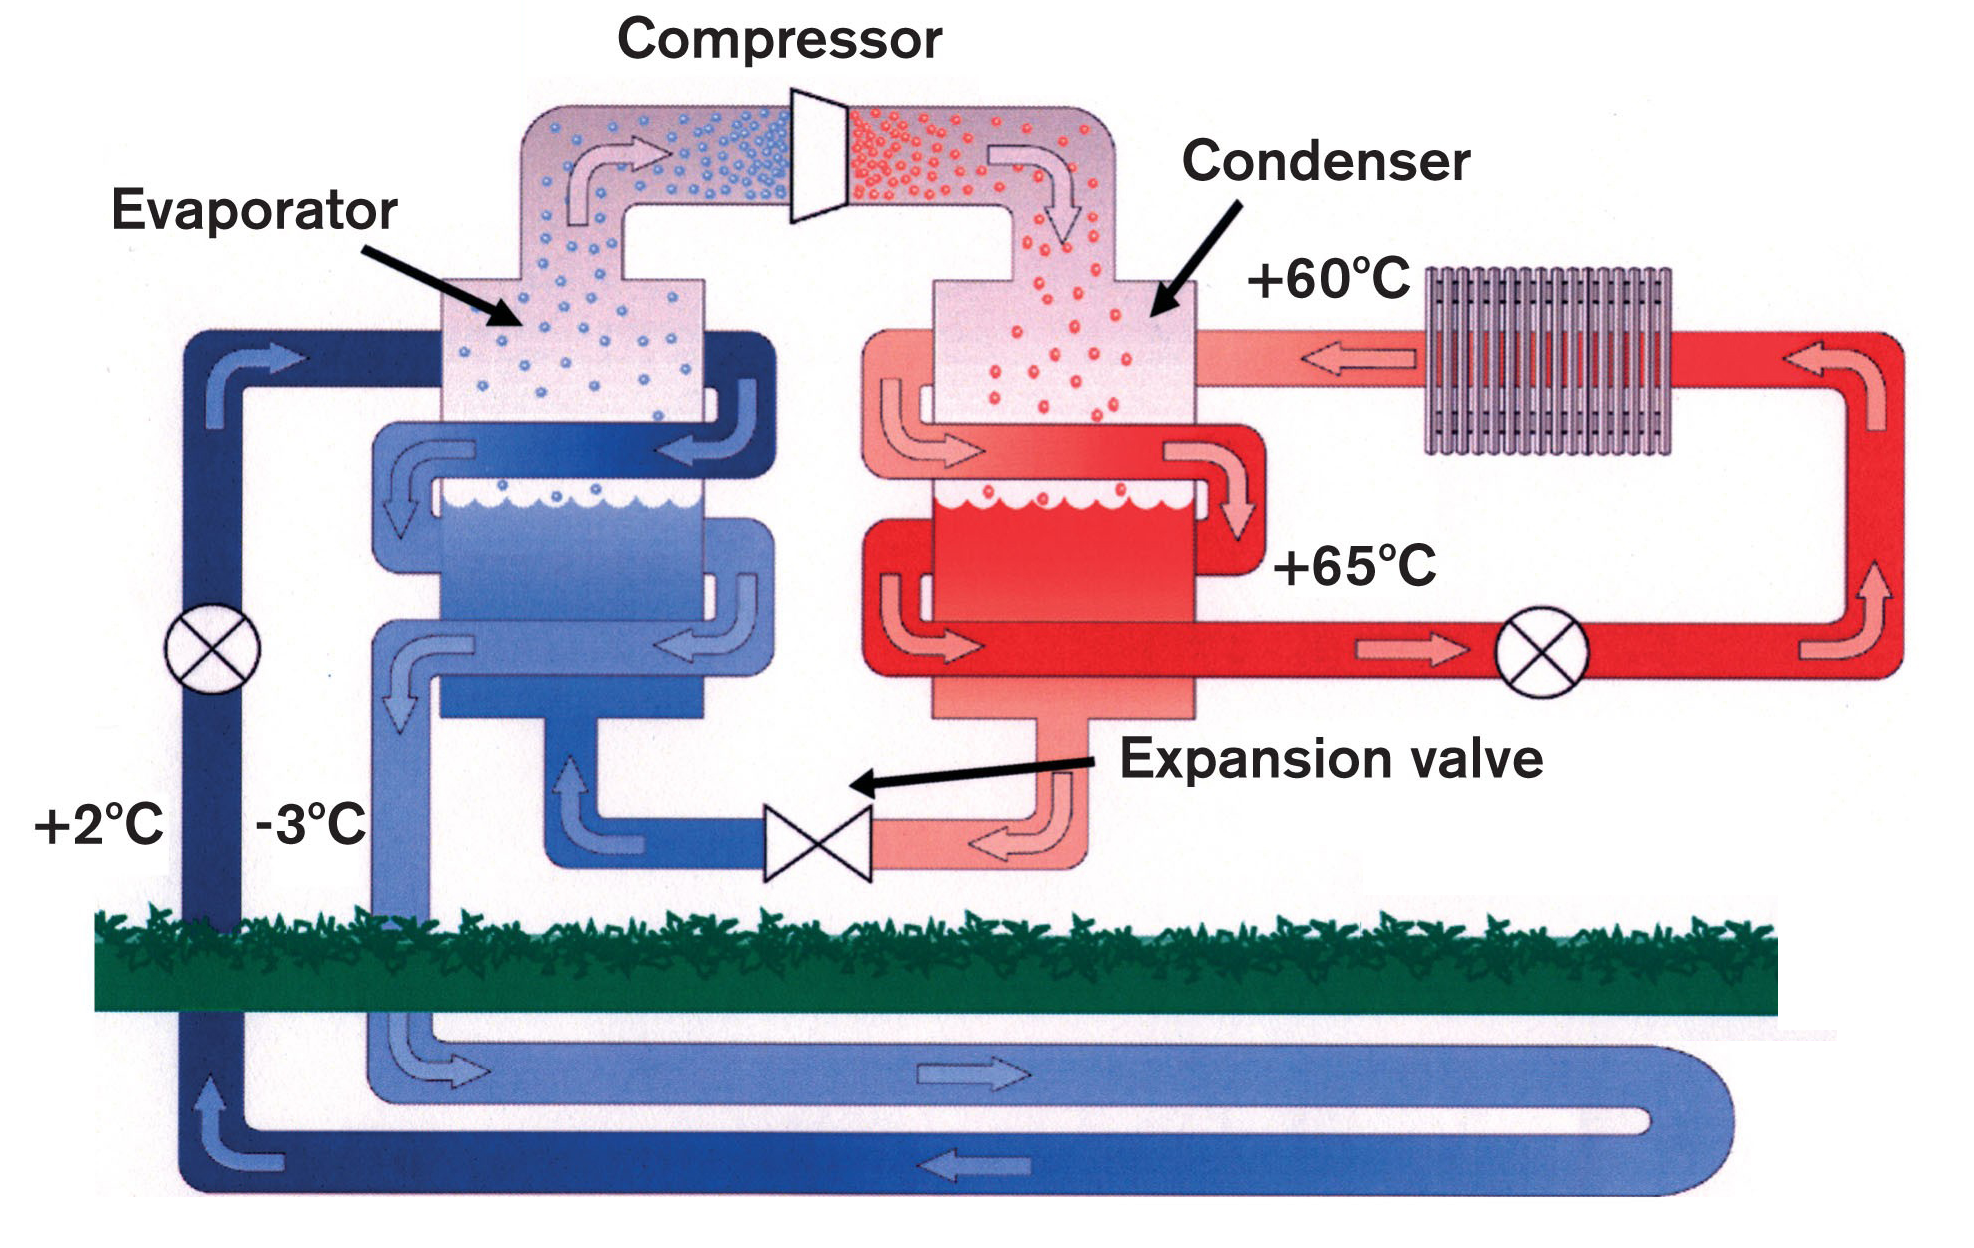
\includegraphics[width=4in]{pictures/Geothermal-Heatpump.png}
    \caption{Implementation of geothermal heat pump in a winter configuration. \textit{Bay Star Energy \cite{HowHeatPumpWorks}}}
\end{figure}
%
\noindent
As seen above, for a winter cycle, the ground is used to heat a working fluid that goes through a loop in the ground. This fluid then goes through a heat exchanger to give the heat into the normal heat pump cycle. The heat pump cycle remains unchanged besides from this replacement of the outdoor physical heat pump with a underground loop system.